\documentclass[12pt,a4paper]{article}

% ─── Page Layout ───────────────────────────────────────────────────────────────
\usepackage[a4paper, margin=0.8in, headheight=14pt]{geometry}

% ─── Fonts (XeLaTeX) ───────────────────────────────────────────────────────────
\usepackage{fontspec}
\usepackage{unicode-math}
\setmainfont{TeX Gyre Pagella}
\setmonofont[Scale=0.88]{TeX Gyre Cursor}
\setmathfont{Latin Modern Math}

% ─── Packages ──────────────────────────────────────────────────────────────────
\usepackage{xcolor}
\usepackage{colortbl}
\usepackage{titlesec}
\usepackage{enumitem}
\usepackage{tabularx}
\usepackage{booktabs}
\usepackage{array}
\usepackage{amsmath}
\usepackage{tikz}
\usetikzlibrary{shapes.geometric, arrows.meta, positioning, calc, fit, decorations.pathreplacing}
\usepackage{tcolorbox}
\tcbuselibrary{skins, breakable}
\usepackage{hyperref}
\usepackage{fancyhdr}
\usepackage{graphicx}
\usepackage{microtype}
\hyphenpenalty=10000
\exhyphenpenalty=10000
\sloppy
\usepackage{caption}
\usepackage{setspace}
\usepackage{multirow}
\usepackage{tocloft}

% ─── Q&A helper ────────────────────────────────────────────────────────────────
\newcommand{\Q}[1]{\textbf{#1}\par\noindent\ignorespaces}

% ─── Colour Palette ────────────────────────────────────────────────────────────
\definecolor{myred}{RGB}{196,30,58}
\definecolor{mydark}{RGB}{30,30,50}
\definecolor{mygreen}{RGB}{14,120,80}
\definecolor{myteal}{RGB}{0,130,140}
\definecolor{myamber}{RGB}{180,100,0}
\definecolor{mypurple}{RGB}{100,30,160}
\definecolor{mygray}{RGB}{246,247,249}
\definecolor{mgframe}{RGB}{180,185,200}
\definecolor{watermark}{RGB}{145,150,170}
\definecolor{hdrred}{RGB}{250,232,235}
\definecolor{hdrgreen}{RGB}{220,244,233}
\definecolor{hdrteal}{RGB}{220,242,244}
\definecolor{hdramber}{RGB}{253,242,215}
\definecolor{hdrpurple}{RGB}{238,228,255}
\definecolor{hdrgray}{RGB}{238,240,245}
\definecolor{rowalt}{RGB}{250,251,253}

% ─── Section Formatting ────────────────────────────────────────────────────────
\titleformat{\section}
  {\large\bfseries\color{myred}}{\thesection.}{0.5em}{}
  [\vspace{1pt}{\color{myred}\rule{\linewidth}{0.8pt}}]
\titleformat{\subsection}
  {\normalsize\bfseries\color{myteal}}{\thesubsection}{0.5em}{}
\titlespacing*{\section}{0pt}{18pt}{7pt}
\titlespacing*{\subsection}{0pt}{11pt}{4pt}

% ─── Paragraph ─────────────────────────────────────────────────────────────────
\setlength{\parindent}{0pt}
\setlength{\parskip}{4pt}

% ─── TOC Styling ───────────────────────────────────────────────────────────────
\renewcommand{\cfttoctitlefont}{\large\bfseries\color{myred}}
\renewcommand{\cftaftertoctitle}{\par\noindent{\color{myred}\rule{\linewidth}{0.8pt}}}
\setlength{\cftbeforetoctitleskip}{0pt}
\setlength{\cftaftertoctitleskip}{6pt}
\renewcommand{\cftsecfont}{\normalsize\bfseries\color{mydark}}
\renewcommand{\cftsecpagefont}{\normalsize\bfseries\color{mydark}}
\renewcommand{\cftsecleader}{\cftdotfill{\cftdotsep}}
\setlength{\cftbeforesecskip}{7pt}
\renewcommand{\cftsubsecfont}{\small\color{mydark}}
\renewcommand{\cftsubsecpagefont}{\small\color{mydark}}
\setlength{\cftbeforesubsecskip}{3pt}
\setlength{\cftsubsecindent}{1.4em}

% ─── Table helpers ─────────────────────────────────────────────────────────────
\renewcommand{\arraystretch}{1.45}
\setlength{\tabcolsep}{6pt}
\arrayrulecolor{mydark}
\newcolumntype{B}[1]{>{\small\bfseries\raggedright\arraybackslash}m{#1}}
\newcolumntype{Y}{>{\small\raggedright\arraybackslash}X}
\renewcommand{\tabularxcolumn}[1]{m{#1}}

% ─── Header / Footer ───────────────────────────────────────────────────────────
\pagestyle{fancy}
\fancyhf{}
\fancyhead[L]{\small\color{myred}\textbf{PE-EC703A}\;\color{mydark}--- Embedded System}
\fancyhead[R]{\small\color{myteal}\textbf{Module 5 Notes}}
\fancyfoot[C]{\small\color{mydark}\thepage}
\fancyfoot[R]{\small\color{watermark}\textit{\copyright\ Biraj}}
\renewcommand{\headrulewidth}{0.5pt}
\renewcommand{\footrulewidth}{0.3pt}

% ─── Hyperref ──────────────────────────────────────────────────────────────────
\hypersetup{
  colorlinks=true, linkcolor=myteal, urlcolor=myteal,
  pdfauthor={Biraj Sarkar},
  pdftitle={PE-EC703A --- Module 5 Notes}
}

% ─── tcolorbox styles ──────────────────────────────────────────────────────────
\tcbset{
  tikzbox/.style={
    colback=mygray, colframe=mgframe, boxrule=0.6pt, arc=4pt,
    left=8pt, right=8pt, top=6pt, bottom=6pt,
    colbacktitle=mgframe, coltitle=mydark,
    fonttitle=\small\bfseries
  },
  defbox/.style={
    colback=hdrgreen, colframe=mygreen, boxrule=0.8pt, arc=4pt,
    left=9pt, right=9pt, top=6pt, bottom=6pt,
    colbacktitle=mygreen, coltitle=white,
    fonttitle=\small\bfseries
  },
  formulabox/.style={
    colback=hdrteal, colframe=myteal, boxrule=0.8pt, arc=4pt,
    left=9pt, right=9pt, top=7pt, bottom=7pt,
    colbacktitle=myteal, coltitle=white,
    fonttitle=\small\bfseries
  },
  examplebox/.style={
    colback=hdramber, colframe=myamber, boxrule=0.8pt, arc=4pt,
    left=9pt, right=9pt, top=6pt, bottom=6pt,
    colbacktitle=myamber, coltitle=white,
    fonttitle=\small\bfseries
  },
  masonbox/.style={
    colback=hdrpurple, colframe=mypurple, boxrule=0.8pt, arc=4pt,
    left=9pt, right=9pt, top=6pt, bottom=6pt,
    colbacktitle=mypurple, coltitle=white,
    fonttitle=\small\bfseries
  },
  exambox/.style={
    colback=hdrpurple, colframe=mypurple, boxrule=1pt, arc=5pt,
    left=10pt, right=10pt, top=8pt, bottom=8pt,
    colbacktitle=mypurple, coltitle=white,
    fonttitle=\bfseries,
    breakable, title after break={\textbf{Frequently Asked / Viva Questions (contd.)}}}
}
\tcbset{breakable}

% ─── TikZ styles ───────────────────────────────────────────────────────────────
\tikzset{
  block/.style={rectangle, draw=myteal, fill=hdrteal,
    text width=2.4cm, align=center, minimum height=0.95cm,
    font=\small, rounded corners=3pt, line width=0.7pt},
  redblock/.style={rectangle, draw=myred, fill=hdrred,
    text width=2.4cm, align=center, minimum height=0.95cm,
    font=\small, rounded corners=3pt, line width=0.7pt},
  netnode/.style={rectangle, draw=myteal, fill=hdrteal,
    text width=1.5cm, align=center, minimum height=0.8cm,
    font=\small, rounded corners=3pt, line width=0.7pt},
  sumjunc/.style={circle, draw=myamber, fill=hdramber,
    minimum size=0.62cm, font=\small, line width=0.8pt},
  snode/.style={circle, draw=mypurple, fill=hdrpurple,
    minimum size=0.55cm, font=\footnotesize, line width=0.7pt},
  arrow/.style={-Stealth, thick, color=mydark},
  redarrow/.style={-Stealth, thick, color=myred},
  line/.style={thick, color=mydark}
}

% ═══════════════════════════════════════════════════════════════════════════════
\begin{document}
% ═══════════════════════════════════════════════════════════════════════════════

\begin{center}
  {\LARGE\bfseries\color{myred} PE-EC703A --- Embedded System}\\[5pt]
  {\normalsize\color{mydark} Semester VII \quad$\bullet$\quad 3L:0T:0P \quad$\bullet$\quad 3 Credits}\\[3pt]
  {\normalsize\color{myteal}\textbf{Module 5 Exam Notes: Embedded System Design using PIC Microcontroller}}\\[3pt]
  {\small\color{mydark} CGEC \;$|$\; B.Tech ECE (2023--27) \;$|$\; \textit{Biraj Sarkar}}
\end{center}
\vspace{2pt}
\noindent{\color{myred}\rule{\linewidth}{1.5pt}}
\vspace{2pt}

\hypersetup{linkcolor=mydark}
\tableofcontents
\hypersetup{linkcolor=myteal}
\newpage

% ===============================================================================
\section{Introduction to Microchip PIC16 Family}
% ===============================================================================

\begin{tcolorbox}[defbox, title={\textbf{PIC Microcontroller}}]
\textbf{PIC} (Peripheral Interface Controller) is a family of microcontrollers manufactured by \textbf{Microchip Technology}. PIC microcontrollers are known for their RISC-based Harvard architecture, a small instruction set ($<$35 instructions for mid-range PIC), low cost, wide voltage range (2.0--5.5 V), and abundant peripheral integration. They are widely used in hobbyist and industrial embedded applications.
\end{tcolorbox}

\subsection{PIC Architecture Classifications}

\par\noindent
{\renewcommand{\arraystretch}{1.6}%
\begin{tabularx}{\linewidth}{|B{3.0cm}|Y|Y|Y|}
\hline
\textbf{Family} & \textbf{Program Word} & \textbf{Data Bus} & \textbf{Examples} \\
\hline
\textbf{PIC10 (Base)} & 12-bit & 8-bit & PIC10F200, PIC10F220 \\
\hline
\textbf{PIC12 (Base)} & 12-bit & 8-bit & PIC12F508, PIC12F675 \\
\hline
\textbf{PIC16 (Mid-range)} & 14-bit & 8-bit & PIC16F84A, PIC16F877A, PIC16F873 \\
\hline
\textbf{PIC18 (Enhanced)} & 16-bit & 8-bit & PIC18F4550, PIC18F452 \\
\hline
\textbf{PIC24 / dsPIC} & 24-bit & 16-bit & dsPIC33, PIC24FJ \\
\hline
\textbf{PIC32} & 32-bit MIPS & 32-bit & PIC32MX, PIC32MZ \\
\hline
\end{tabularx}}

\subsection{Key Architectural Features of PIC Mid-Range (PIC16)}
\begin{itemize}[leftmargin=*, itemsep=3pt]
  \item \textbf{Harvard Architecture:} Separate program (Flash) and data (RAM + SFR) buses.
  \item \textbf{RISC Core:} Only 35 instructions; most execute in 1 instruction cycle (4 clock cycles).
  \item \textbf{Instruction Cycle:} $T_{cy} = 4 / f_{OSC}$ (e.g., at 20 MHz: $T_{cy} = 200\,\text{ns}$).
  \item \textbf{8-bit Working Register (W):} Equivalent to the Accumulator in 8051.
  \item \textbf{File Register Architecture:} All RAM, SFRs, and I/O registers accessed via ``file register'' addresses.
  \item \textbf{Pipelining:} 2-stage pipeline (Fetch + Execute) --- while one instruction executes, the next is fetched.
\end{itemize}

\begin{tcolorbox}[formulabox, title={\textbf{PIC16 Key Formulas}}]
\[
T_{cy} = \frac{4}{f_{OSC}} \qquad (\text{1 instruction cycle} = 4 \text{ clock periods})
\]
\[
\text{Timer0 Overflow Time} = \frac{(256 - \text{TMR0}) \times \text{Prescaler} \times 4}{f_{OSC}}
\]
\[
\text{ADC Resolution} = \frac{V_{REF}}{2^N - 1} \quad (N = 10\text{ bits for PIC16F873})
\]
\[
\text{Baud Rate (UART)} = \frac{f_{OSC}}{64 \times (\text{SPBRG} + 1)} \quad (\text{Low speed mode})
\]
\end{tcolorbox}

% ===============================================================================
\section{PIC16F873 --- Architecture and Features}
% ===============================================================================

\begin{tcolorbox}[defbox, title={\textbf{PIC16F873}}]
The \textbf{PIC16F873} is a 28-pin Flash-based mid-range PIC microcontroller from Microchip. It is a popular choice for educational and industrial embedded designs due to its integrated analog and communication peripherals, Flash programmability, and low power consumption.
\end{tcolorbox}

\subsection{PIC16F873 --- Key Specifications}

\par\noindent
{\renewcommand{\arraystretch}{1.55}%
\begin{tabularx}{\linewidth}{|B{3.5cm}|Y|}
\hline
\textbf{Feature} & \textbf{Specification} \\
\hline
\textbf{Program Memory} & 8 KB Flash (4096 x 14-bit words) \\
\hline
\textbf{Data Memory (RAM)} & 192 bytes SRAM \\
\hline
\textbf{Data EEPROM} & 128 bytes \\
\hline
\textbf{I/O Ports} & PORTA (6 pins), PORTB (8 pins), PORTC (8 pins) = 22 I/O \\
\hline
\textbf{Timers} & Timer0 (8-bit), Timer1 (16-bit), Timer2 (8-bit + PR2) \\
\hline
\textbf{ADC} & 5-channel, 10-bit ADC (AN0--AN4 on PORTA) \\
\hline
\textbf{Serial Ports} & USART (UART/SPI async), MSSP (SPI + I2C) \\
\hline
\textbf{Interrupts} & Up to 13 interrupt sources \\
\hline
\textbf{Clock Speed} & DC to 20 MHz (using external crystal) \\
\hline
\textbf{Supply Voltage} & 2.0 V to 5.5 V \\
\hline
\textbf{Package} & 28-pin PDIP, SOIC, SSOP \\
\hline
\textbf{Watchdog Timer} & Built-in WDT with independent RC oscillator \\
\hline
\end{tabularx}}

\begin{tcolorbox}[tikzbox, title={PIC16F873 Block Diagram}]
\centering
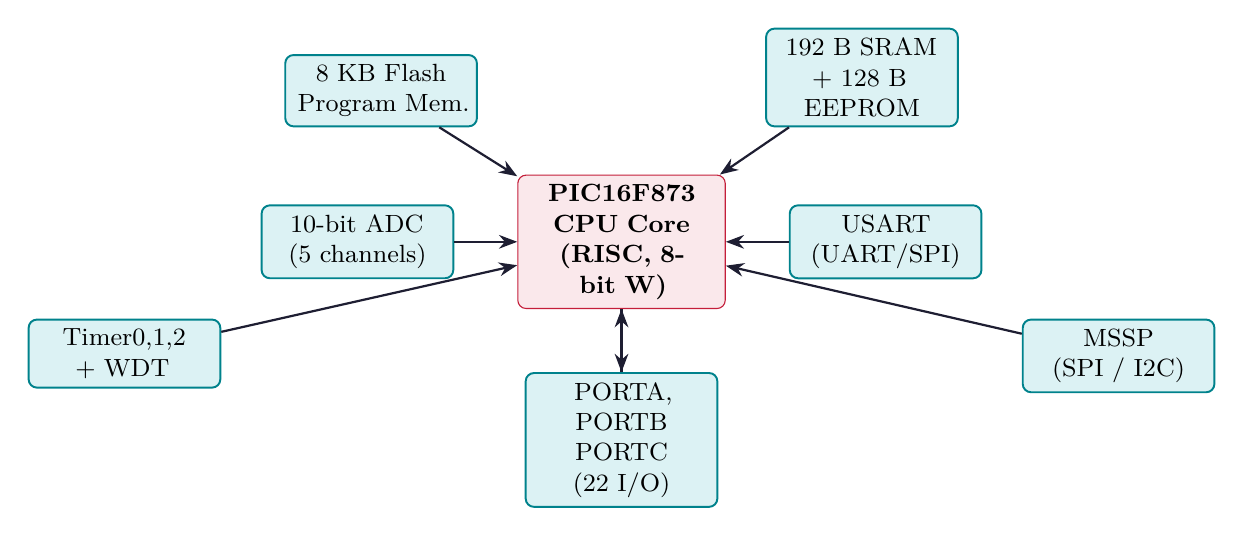
\begin{tikzpicture}[node distance=0.35cm and 0.6cm,
  sblock/.style={rectangle, draw=myteal, fill=hdrteal, text width=2.2cm,
    align=center, minimum height=0.75cm, font=\small, rounded corners=3pt, line width=0.7pt}]
  % Central CPU
  \node[rectangle, draw=myred, fill=hdrred, text width=2.4cm, align=center,
    minimum height=1.0cm, font=\small\bfseries, rounded corners=3pt] (cpu) {PIC16F873\\CPU Core\\(RISC, 8-bit W)};

  % Memory
  \node[sblock, above left=0.6cm and 0.5cm of cpu] (flash) {8 KB Flash\\Program Mem.};
  \node[sblock, above right=0.6cm and 0.5cm of cpu] (sram) {192 B SRAM\\+ 128 B EEPROM};

  % Peripherals left
  \node[sblock, left=0.8cm of cpu] (adc) {10-bit ADC\\(5 channels)};
  \node[sblock, below left=0.5cm and 0.5cm of adc] (tmr) {Timer0,1,2\\+ WDT};

  % Peripherals right
  \node[sblock, right=0.8cm of cpu] (usart) {USART\\(UART/SPI)};
  \node[sblock, below right=0.5cm and 0.5cm of usart] (mssp) {MSSP\\(SPI / I2C)};

  % I/O
  \node[sblock, below=0.8cm of cpu] (io) {PORTA, PORTB\\PORTC (22 I/O)};

  \draw[arrow] (flash) -- (cpu);
  \draw[arrow] (sram) -- (cpu);
  \draw[arrow] (adc) -- (cpu);
  \draw[arrow] (tmr) -- (cpu);
  \draw[arrow] (usart) -- (cpu);
  \draw[arrow] (mssp) -- (cpu);
  \draw[arrow] (io) -- (cpu);
  \draw[arrow] (cpu) -- (io);
\end{tikzpicture}
\end{tcolorbox}

% ===============================================================================
\section{On-Chip Peripherals of PIC16F873}
% ===============================================================================

\subsection{Watchdog Timer (WDT)}
\begin{itemize}[leftmargin=*, itemsep=3pt]
  \item Has its own internal \textbf{RC oscillator} (independent of main clock); continues running even if main clock fails.
  \item Default timeout period $\approx$ 18 ms; extended via \textbf{postscaler} (up to $\times 128$ $\approx$ 2.3 s).
  \item Reset by \texttt{CLRWDT} instruction in software.
  \item On timeout: generates a device reset (MCLR pin goes low momentarily).
  \item Can be enabled/disabled via configuration word bits.
\end{itemize}

\subsection{ADC (Analog-to-Digital Converter)}
\begin{itemize}[leftmargin=*, itemsep=3pt]
  \item \textbf{10-bit successive approximation ADC}: Converts analog voltage to a 10-bit digital value (0 to 1023).
  \item \textbf{5 analog input channels} (AN0--AN4) on PORTA (multiplexed with digital I/O).
  \item \textbf{Reference voltage:} $V_{REF+}$ and $V_{REF-}$ pins (or $V_{DD}$ and $V_{SS}$ by default).
  \item \textbf{Acquisition time:} Capacitor sampling time before conversion starts; minimum 2 $\mu$s.
  \item \textbf{Result format:} Left-justified or right-justified; stored in ADRESH:ADRESL registers.
\end{itemize}

\begin{tcolorbox}[examplebox, title={\textbf{PIC16F873 ADC --- Conversion Steps}}]
\begin{enumerate}[topsep=0pt, leftmargin=*, itemsep=2pt]
  \item Configure ADCON1 (select analog/digital pin assignment and $V_{REF}$).
  \item Configure ADCON0 (select channel AN$x$, clock source, turn ADC ON).
  \item Wait for acquisition time ($\geq 2\,\mu$s).
  \item Set \texttt{GO/DONE} bit in ADCON0 to start conversion.
  \item Poll \texttt{GO/DONE} bit until it clears (conversion complete, $\approx 12 \times T_{AD}$).
  \item Read 10-bit result from \texttt{ADRESH} (high 2 bits) and \texttt{ADRESL} (low 8 bits).
\end{enumerate}
\end{tcolorbox}

\subsection{Asynchronous Serial Port --- USART}
\begin{itemize}[leftmargin=*, itemsep=3pt]
  \item Full-duplex UART on RC6 (TX) and RC7 (RX).
  \item Baud rate controlled by SPBRG register and BRGH bit (high/low speed).
  \item \textbf{High-speed mode (BRGH=1):} $\text{Baud} = f_{OSC} / (16 \times (\text{SPBRG}+1))$
  \item \textbf{Low-speed mode (BRGH=0):} $\text{Baud} = f_{OSC} / (64 \times (\text{SPBRG}+1))$
  \item Interrupt flags: TXIF (transmit buffer empty), RCIF (receive buffer full).
\end{itemize}

\subsection{SPI and I2C --- MSSP Module}
\begin{itemize}[leftmargin=*, itemsep=3pt]
  \item The \textbf{MSSP} (Master Synchronous Serial Port) supports both SPI and I2C modes.
  \item \textbf{SPI Mode:} Uses RC3 (SCK), RC4 (SDI), RC5 (SDO), and any GPIO as CS (Chip Select). Master or slave configurable.
  \item \textbf{I2C Mode:} Uses RC3 (SCL) and RC4 (SDA) with open-drain outputs. Supports 7-bit and 10-bit addressing.
\end{itemize}

% ===============================================================================
\section{Interfacing with PIC16F873}
% ===============================================================================

\subsection{LCD Interfacing}

\begin{tcolorbox}[defbox, title={\textbf{LCD (16$\times$2) Interfacing with PIC16F873}}]
A standard Hitachi HD44780-compatible 16$\times$2 character LCD is interfaced using \textbf{4-bit mode} (4 data lines + 3 control lines) to save I/O pins. Control pins: RS (Register Select: 0=Command, 1=Data), RW (Read/Write, tied to GND for write-only), EN (Enable pulse to latch data).
\end{tcolorbox}

\begin{tcolorbox}[tikzbox, title={PIC16F873 to 16$\times$2 LCD --- 4-bit Interface}]
\centering
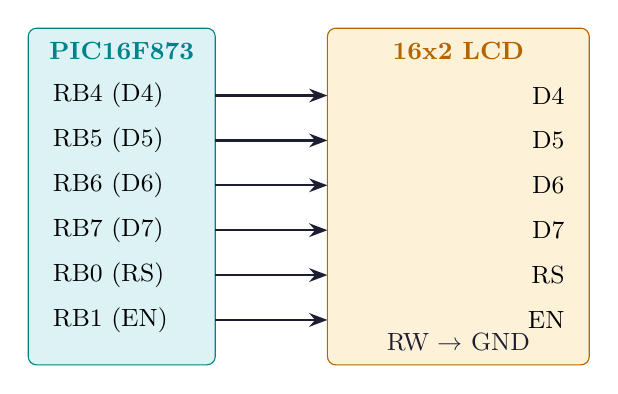
\begin{tikzpicture}[scale=0.95, every node/.style={font=\small}]
  % PIC block
  \draw[fill=hdrteal, draw=myteal, rounded corners=3pt] (0, 0) rectangle (2.5, 4.5);
  \node[font=\small\bfseries, color=myteal] at (1.25, 4.2) {PIC16F873};
  \node[right] at (0.2, 3.6) {RB4 (D4)};
  \node[right] at (0.2, 3.0) {RB5 (D5)};
  \node[right] at (0.2, 2.4) {RB6 (D6)};
  \node[right] at (0.2, 1.8) {RB7 (D7)};
  \node[right] at (0.2, 1.2) {RB0 (RS)};
  \node[right] at (0.2, 0.6) {RB1 (EN)};

  % Connections
  \foreach \y in {3.6, 3.0, 2.4, 1.8, 1.2, 0.6}
    \draw[arrow] (2.5, \y) -- (4.0, \y);

  % LCD block
  \draw[fill=hdramber, draw=myamber, rounded corners=3pt] (4.0, 0) rectangle (7.5, 4.5);
  \node[font=\small\bfseries, color=myamber] at (5.75, 4.2) {16x2 LCD};
  \node[left] at (7.3, 3.6) {D4};
  \node[left] at (7.3, 3.0) {D5};
  \node[left] at (7.3, 2.4) {D6};
  \node[left] at (7.3, 1.8) {D7};
  \node[left] at (7.3, 1.2) {RS};
  \node[left] at (7.3, 0.6) {EN};
  \node[font=\small, color=mydark] at (5.75, 0.3) {RW $\to$ GND};
\end{tikzpicture}
\end{tcolorbox}

\subsection{ADC Interfacing (Sensors)}
\begin{itemize}[leftmargin=*, itemsep=3pt]
  \item Temperature sensor (LM35): Output voltage = 10 mV/$^\circ$C. Connect to AN0.
    \begin{itemize}
      \item ADC result $\to$ Temperature: $T(^{\circ}C) = \frac{\text{ADC} \times V_{REF}}{1023 \times 0.01}$
    \end{itemize}
  \item Potentiometer / Joystick: Directly connected to analog input (voltage divider).
  \item Light sensor (LDR): Used in voltage divider; ADC reads light level.
\end{itemize}

\subsection{Stepper Motor Interfacing}
\begin{itemize}[leftmargin=*, itemsep=3pt]
  \item A stepper motor advances by a fixed angle (step) for each control pulse.
  \item \textbf{Step angle:} Depends on motor type (e.g., $1.8^\circ$/step = 200 steps/revolution).
  \item \textbf{Driver IC:} L298N or ULN2003 connects between PIC output pins and motor coils.
  \item PIC sends sequence of bit patterns to PORTB to rotate the stepper.
  \item \textbf{Full-step sequence (4-phase):} 1100 $\to$ 0110 $\to$ 0011 $\to$ 1001 (repeat).
\end{itemize}

\subsection{Keyboard (Keypad) Interfacing}
\begin{itemize}[leftmargin=*, itemsep=3pt]
  \item A \textbf{4$\times$4 matrix keypad} uses 4 row + 4 column lines = 8 pins.
  \item PIC drives rows LOW one at a time, then reads which column line goes LOW.
  \item The row/column combination identifies the pressed key.
  \item Debouncing: Software delay ($\sim$20 ms) after detecting key press before confirming it.
\end{itemize}

\subsection{DAC (Digital-to-Analog Converter)}
\begin{itemize}[leftmargin=*, itemsep=3pt]
  \item PIC16F873 has no built-in DAC. External options:
    \begin{itemize}
      \item \textbf{R-2R Resistor Ladder:} Passive DAC using resistors connected to PORTB (8-bit). Simple, low cost, no extra IC.
      \item \textbf{External DAC IC (MCP4921):} 12-bit DAC with SPI interface.
      \item \textbf{PWM + RC filter:} Use Timer2 PWM output, filter with RC low-pass $\to$ analog voltage proportional to duty cycle.
    \end{itemize}
\end{itemize}

% ===============================================================================
\section{Case Studies of Embedded System Design}
% ===============================================================================

\subsection{Case Study 1: Automated Chocolate Vending Machine}

\begin{tcolorbox}[examplebox, title={\textbf{Automated Chocolate Vending Machine using PIC16F873}}]
\textbf{Problem:} Design a vending machine that accepts coins (detected by IR sensor), displays balance on LCD, dispenses chocolate (stepper motor) when enough coins are inserted, and provides change.

\textbf{Hardware Components:}
\begin{itemize}[leftmargin=*, itemsep=2pt, topsep=4pt]
  \item PIC16F873 (controller), 16$\times$2 LCD (display), IR coin sensor on AN0 (ADC), Stepper motor + ULN2003 (dispenser), Buzzer on RB0 (feedback), Keypad for item selection.
\end{itemize}

\textbf{Software Flow:}
\begin{enumerate}[topsep=4pt, leftmargin=*, itemsep=2pt]
  \item Initialize LCD, ADC, I/O ports.
  \item Display ``Insert Coin'' on LCD.
  \item Loop: Poll coin sensor (ADC reading $>$ threshold $\to$ coin detected).
  \item On coin: Increment balance; update LCD display.
  \item If balance $\geq$ price: Drive stepper motor (4 steps) to dispense; beep buzzer.
  \item Calculate and dispense change (reverse stepper? No --- separate change mechanism).
  \item Reset balance; display ``Thank You''.
\end{enumerate}

\textbf{Key Programming Concepts Used:} ADC polling, stepper motor control sequences, LCD 4-bit mode, software debounce, timer-based delay.
\end{tcolorbox}

\begin{tcolorbox}[tikzbox, title={Vending Machine System Block Diagram}]
\centering
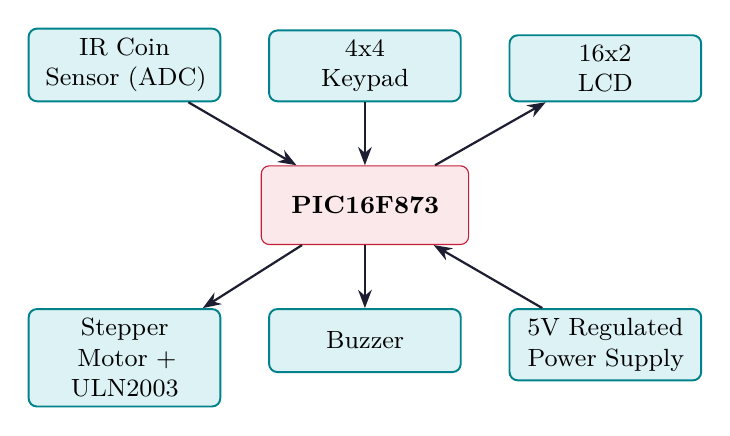
\begin{tikzpicture}[node distance=0.3cm and 0.6cm,
  sblock/.style={rectangle, draw=myteal, fill=hdrteal, text width=2.2cm,
    align=center, minimum height=0.8cm, font=\small, rounded corners=3pt, line width=0.7pt}]
  \node[rectangle, draw=myred, fill=hdrred, text width=2.4cm, align=center,
    minimum height=1.0cm, font=\small\bfseries, rounded corners=3pt] (pic) {PIC16F873};
  \node[sblock, above left=0.8cm and 0.5cm of pic] (coin) {IR Coin\\Sensor (ADC)};
  \node[sblock, above=0.8cm of pic] (keypad) {4x4\\Keypad};
  \node[sblock, above right=0.8cm and 0.5cm of pic] (lcd) {16x2\\LCD};
  \node[sblock, below left=0.8cm and 0.5cm of pic] (motor) {Stepper\\Motor + ULN2003};
  \node[sblock, below=0.8cm of pic] (buzzer) {Buzzer};
  \node[sblock, below right=0.8cm and 0.5cm of pic] (pwr) {5V Regulated\\Power Supply};

  \draw[arrow] (coin) -- (pic);
  \draw[arrow] (keypad) -- (pic);
  \draw[arrow] (pic) -- (lcd);
  \draw[arrow] (pic) -- (motor);
  \draw[arrow] (pic) -- (buzzer);
  \draw[arrow] (pwr) -- (pic);
\end{tikzpicture}
\end{tcolorbox}

\subsection{Case Study 2: Digital Camera Controller}

\begin{tcolorbox}[examplebox, title={\textbf{Digital Camera Controller using PIC (Concept)}}]
\textbf{Note:} A full digital camera uses high-performance processors (e.g., ARM Cortex-A) for image processing. PIC16F873 can implement the \textbf{camera control subsystem} (not image processing).

\textbf{PIC16F873 Role in Digital Camera:}
\begin{itemize}[leftmargin=*, itemsep=2pt, topsep=4pt]
  \item \textbf{Shutter Control:} Timer-based precise shutter speed control (1/1000s to 1/30s) using Timer1 interrupt.
  \item \textbf{Focus Motor Control:} Stepper motor drives lens position; PIC reads ADC from autofocus sensor.
  \item \textbf{Flash Trigger:} GPIO pin triggers external flash unit via optocoupler.
  \item \textbf{User Interface:} Reads mode dial (keypad), displays settings on small LCD.
  \item \textbf{Battery Monitor:} ADC reads battery voltage divider; displays charge level.
  \item \textbf{Serial Communication:} UART or SPI to main image processor (ARM) for command passing.
\end{itemize}

\textbf{Key Techniques:} Timer interrupts for precision timing, ADC for sensor reading, SPI for inter-processor communication, WDT for reliability.
\end{tcolorbox}

% ===============================================================================
% MANDATORY QUICK REVISION PAGE
% ===============================================================================
\newpage
\begin{center}
  {\large\bfseries\color{myred} Quick Revision --- Module 5}\\[3pt]
  {\small\color{mydark} Embedded System Design using PIC Microcontroller $|$ PE-EC703A}
\end{center}
\noindent{\color{myred}\rule{\linewidth}{1.2pt}}
\vspace{4pt}

\begin{tcolorbox}[formulabox, title={\textbf{Key Formulas at a Glance}}]
\renewcommand{\arraystretch}{1.3}
\begin{tabularx}{\linewidth}{B{4.5cm} X}
Instruction Cycle & $T_{cy} = \displaystyle\frac{4}{f_{OSC}}$ \quad (at 20 MHz: $T_{cy} = 200\,\text{ns}$) \\[4pt]
Timer0 Overflow & $t_{TMR0} = \displaystyle\frac{(256 - \text{TMR0\_init}) \times \text{Prescaler} \times 4}{f_{OSC}}$ \\[4pt]
ADC Result (10-bit) & $V_{in} = \displaystyle\frac{\text{ADC} \times V_{REF}}{1023}$ \quad (right-justified) \\[4pt]
UART Baud (BRGH=1) & $\text{Baud} = \displaystyle\frac{f_{OSC}}{16 \times (\text{SPBRG}+1)}$ \\[4pt]
ADC Temperature (LM35) & $T(^{\circ}\text{C}) = \displaystyle\frac{\text{ADC} \times V_{REF}}{1023 \times 0.01}$
\end{tabularx}
\end{tcolorbox}

\begin{tcolorbox}[defbox, title={\textbf{One-Line Definitions}}]
\begin{itemize}[leftmargin=*, itemsep=2.5pt, topsep=0pt]
  \item \textbf{PIC:} Peripheral Interface Controller --- Microchip Technology's RISC-based MCU family.
  \item \textbf{PIC16F873:} 28-pin, 8-bit Flash PIC MCU; 8 KB Flash, 192 B SRAM, 10-bit ADC, USART, MSSP.
  \item \textbf{W Register:} Working Register in PIC --- equivalent to Accumulator; all ALU operations use W.
  \item \textbf{File Register:} PIC's general-purpose RAM + SFR memory, accessed via file register addresses.
  \item \textbf{ADCON0/1:} ADC Control registers in PIC16F873 that configure channel selection, clock, and reference.
  \item \textbf{MSSP:} Master Synchronous Serial Port --- supports SPI and I2C in PIC16F873.
  \item \textbf{USART:} Universal Synchronous/Asynchronous Receiver/Transmitter --- UART + SPI on PIC.
  \item \textbf{SPBRG:} Serial Port Baud Rate Generator register --- sets UART baud rate in PIC.
  \item \textbf{Prescaler:} Divides the clock signal before reaching the timer --- extends the timer overflow period.
  \item \textbf{TMR0:} 8-bit Timer/Counter in PIC16F873 (overflows at 255 $\to$ 0, generates TMR0IF).
  \item \textbf{CLRWDT:} Assembly instruction to reset the Watchdog Timer in PIC.
  \item \textbf{Full-step sequence:} 4-phase stepper motor control pattern (1100, 0110, 0011, 1001).
\end{itemize}
\end{tcolorbox}

\begin{tcolorbox}[exambox, title={\textbf{Frequently Asked / Viva Questions}}]
\begin{enumerate}[topsep=0pt, label=\textbf{Q\arabic*.}, itemsep=5pt]
  \item \Q{What does PIC stand for and who manufactures it?}
    PIC stands for \textbf{Peripheral Interface Controller}. It is manufactured by \textbf{Microchip Technology Inc.}
  \item \Q{State the key features of PIC16F873.}
    28-pin PDIP; 8 KB Flash program memory; 192 B SRAM; 128 B EEPROM; 10-bit 5-channel ADC; three timers (Timer0/1/2); USART; MSSP (SPI + I2C); up to 20 MHz clock; 2.0--5.5 V supply; built-in WDT.
  \item \Q{What is the W register in PIC? How is it different from 8051's Accumulator?}
    The \textbf{W (Working) register} is PIC's primary data register used for ALU operations. Similar to the Accumulator in 8051, it is used as the source/destination for most arithmetic and logic instructions. Unlike 8051's A, W is not directly addressable in the file register map.
  \item \Q{What is the instruction cycle of PIC16 and how does it relate to clock frequency?}
    One instruction cycle = 4 clock cycles: $T_{cy} = 4/f_{OSC}$. At 20 MHz, $T_{cy} = 200\,\text{ns}$. Most PIC instructions execute in 1 cycle (200 ns); branch instructions take 2 cycles.
  \item \Q{How does the PIC16F873 ADC work? What is the resolution?}
    It is a 10-bit successive approximation ADC. It samples the analog voltage on AN0--AN4, converts it to a 10-bit number (0--1023) representing $V_{in}$ between $V_{REF-}$ and $V_{REF+}$. Resolution = $V_{REF}/1023$ (e.g., $\approx 4.88\,\text{mV}$ for 5V reference).
  \item \Q{Explain how a stepper motor is interfaced with PIC16F873.}
    The PIC outputs a 4-bit step sequence to PORTB (e.g., 1100, 0110, 0011, 1001 for full-step mode). Each pattern energizes the motor coils in sequence. A ULN2003 Darlington driver IC between PORTB and the motor coils amplifies the current. The step rate (delay between patterns) controls motor speed.
  \item \Q{What is the difference between USART and MSSP in PIC16F873?}
    \textbf{USART:} Handles asynchronous serial (UART) and synchronous serial (SPI) communication on RC6/RC7. \textbf{MSSP:} A second serial module supporting both SPI (master/slave) and I2C master/slave modes on RC3/RC4/RC5. Both can be used simultaneously.
  \item \Q{How is LCD interfaced with PIC16F873 in 4-bit mode?}
    Only 4 data lines (D4--D7) are connected to PORTB, along with RS and EN control lines (RW tied to GND). Data is sent as two 4-bit nibbles (high nibble first, then low nibble), each latched by pulsing EN high then low.
  \item \Q{How does the Watchdog Timer work in PIC16F873?}
    The WDT has its own RC oscillator ($\approx$18 ms period). Software must execute \texttt{CLRWDT} instruction before timeout. If not cleared in time (e.g., due to program hang), WDT causes a device reset. Timeout can be extended using a postscaler (up to $\times 128 \approx 2.3\,\text{s}$).
  \item \Q{What are the Timer modes available in PIC16F873?}
    \textbf{Timer0:} 8-bit timer/counter with prescaler (1:2 to 1:256). \textbf{Timer1:} 16-bit timer/counter, can use external crystal for low-power RTC. \textbf{Timer2:} 8-bit timer with prescaler and postscaler; period register PR2 sets overflow point; used for PWM generation.
  \item \Q{Describe the design of an automated vending machine using PIC16F873.}
    \begin{itemize}[leftmargin=*, itemsep=1pt, topsep=2pt]
      \item IR sensor (ADC) detects coins; balance tracked in SRAM variable.
      \item LCD (4-bit mode) shows balance and prompts.
      \item Keypad selects product; price compared with balance.
      \item If balance $\geq$ price: stepper motor (via ULN2003) dispenses product; buzzer beeps.
      \item Balance decremented by price; ``Thank You'' displayed.
    \end{itemize}
  \item \Q{Why is PIC preferred for cost-sensitive embedded applications?}
    PIC MCUs are very inexpensive (PIC16F84A $\sim$ Rs.~80--160), available in small packages, have wide voltage range (2--5.5 V), abundant development tools (MPLAB IDE, free compiler), large community, and integrate all needed peripherals on-chip (eliminating external ICs). They are ideal for high-volume, cost-sensitive consumer products.
\end{enumerate}
\end{tcolorbox}

\begin{tcolorbox}[tikzbox, title={PIC16F873 vs.\ 8051 vs.\ ARM Cortex-M0 --- Comparison}]
\par\noindent
{\renewcommand{\arraystretch}{1.55}%
\begin{tabularx}{\linewidth}{|B{2.5cm}|Y|Y|Y|}
\hline
\textbf{Feature} & \textbf{PIC16F873} & \textbf{8051 (AT89S52)} & \textbf{ARM Cortex-M0} \\
\hline
\textbf{Architecture} & Harvard RISC (8-bit) & Harvard CISC (8-bit) & Harvard RISC (32-bit) \\
\hline
\textbf{Instructions} & 35 (14-bit words) & 255 (variable) & Thumb-2 (16/32-bit) \\
\hline
\textbf{Max Clock} & 20 MHz & 33 MHz & 48 MHz \\
\hline
\textbf{Flash} & 8 KB & 8 KB (ISP) & 32--128 KB \\
\hline
\textbf{RAM} & 192 bytes & 256 bytes & 8--32 KB \\
\hline
\textbf{Built-in ADC} & 10-bit, 5-ch & None & 12-bit, 8+ ch \\
\hline
\textbf{Price (approx.)} & Rs.~40--160 & Rs.~65--160 & Rs.~80--400 \\
\hline
\textbf{IDE} & MPLAB X & Keil, SDCC & Keil, GCC ARM \\
\hline
\end{tabularx}}
\end{tcolorbox}

\end{document}
